\section{Frontend}\label{sec:impl_frontend}
Frontendová část tohoto projektu zajišťuje především komunikaci mezi uživatelem a serverem pomocí prostředí, díky kterému je tato komunikace snazší a obecně přívětivější. Serverová část očekává příchozí požadavky od této části na cesty, které byly už definovány (viz sekce \ref{sec:routes}).

V rámci této implementace (a z podstaty využitých technologií) probíhá komunikace s API (viz sekce \ref{sec:impl_backend}), které se tato část snaží poskytovat validní data. Slovo \uv{snaží} je zmíněno proto, jelikož se na ni v reálném světe nemůžeme úplně spoléhat - frontendovou část může uživatel s dostatečnými znalostmi a zkušenostmi modifikovat, čímž může i změnit způsob komunikace se serverem. To ale neznamená, že na ní nemůže probíhat jakákoliv validace a kontrola dat - frontend pro správnou funkčnost celé aplikace musí serveru ve výchozím (uživatelem nezměněném) stavu backendu poskytovat validní data - backend je ale musí preventivně validovat taky.

Uživatelské prostředí musí být připraveno tak, aby bylo příjemné k užívání a ergonomické. Zároveň by nemělo být nějak složité a přehlcené ovládacími prvky, což by mohlo uživatele od používání aplikace odradit. Dále by toto prostředí mělo uživatele \uv{vést} úkonem, který chce uživatel provést - tzn. pokud zadává neplatná data, tak ho upozornit a rozhodně počkat na opravu dat před odesláním požadavku na server. Uživatelské prostředí, které v rámci tohoto projektu vzniklo, je určeno primárně pro vykreslování ve webovém prohlížeči.

V následující části jsou popsány jednotlivé frontendové komponenty a principy, díky kterým může celá aplikace fungovat.
	
	\subsection{Obecná struktura VueJS aplikace}\label{sec:obecna_str_vuejs}
	Nejprve je nutné rozebrat obecnou strukturu VueJS projektu.
	
	\begin{figure}[H]
		\centering
		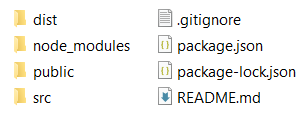
\includegraphics[width=0.6\textwidth]{img/vuejs_struktura.png} 
		\caption{Obecná struktura nově vygenerovaného VueJS projektu}
		\label{fig:vuejs_str}
	\end{figure}

	Jak můžeme na obrázku \ref{fig:vuejs_str} vidět, celý projekt je složen z mnoha složek a souborů. Podrobný rozbor všech souborů a složek není předmětem této práce, proto jsou nejdůležitější zmíněné části popsány níže jen obecně.
	
	\begin{itemize}
		\item Složka \textit{dist} obsahuje zkompilovaný kód aplikace
		\item Složka \textit{node\_modules} obsahuje závislosti a soubory přídavných balíčků NPM (viz sekce \ref{sec:npm}), které aplikace používá
		\item Složka \textit{public} obsahuje obecně veřejné soubory (např. favicon)
		\item Složka \textit{src} obsahuje všechny soubory se zdrojovým kódem, ze kterých se poté tvoří zkompilovaný kód celé aplikace
		\item Soubor \textit{package.json} obsahuje informace o přídavných balíčcích spravovaných pomocí NPM (viz sekce \ref{sec:npm})
	\end{itemize}

	*cite https://5balloons.info/project-tour-of-vue-cli-app/*
	*cite https://stackoverflow.com/questions/22842691/what-is-the-meaning-of-the-dist-directory-in-open-source-projects*
	
	Popsaná struktura výše je standardní pro oddělenou frontendovou aplikaci. To v implementaci tohoto projektu ale neplatí, jelikož je frontend přímo zaintegrován v Laravel projektu (viz sekce \ref{sec:strukura_laravel}). Jsou zde tyto rozdíly:
	
	\begin{itemize}
		\item Složka \textit{src} je nahrazena složkou \textit{js} ve složce \textit{resources}
		\item Složka \textit{public} je umístěna v kořenovém adresáři Laravel projektu a je sloučena se složkou \textit{dist}
		\item Složka \textit{node\_modules} společně se souborem \textit{package.json} je také umístěna v kořenovém adresáři Laravel projektu
	\end{itemize}
	
	Celkovou administrativu nad celým Vue projektem poté zajišťuje modul Laravel Mix podle konfiguračního souboru webpack.mix.js. Ten je také umístěn v kořenovém adresáři projektu. *cite https://laravel-mix.com/docs/6.0/vue* Díky celému tomuto přístupu může backend i frontend běžet jako jedna aplikace na jedné doméně.
	
	Jak již bylo zmíněno, zdrojový kód, tedy nejdůležitější část frontendové aplikace, leží standardně ve složce \textit{src} - v tomto projektu ve zmíněné složce \textit{js}. Oproti běžné samostatné Vue aplikaci je zde (ve složce \textit{js}) největší rozdíl v pojmenování souborů - soubor \textit{main.js} byl přejmenován pro potřeby Laravelu na \textit{app.js}. Také se navíc v této složce nachází Laravelem vygenerovaný soubor bootstrap.js pro další konfiguraci při kompilaci. Nakonec byla kvůli nevyužití odebrána složka \textit{assets} a pro další účely přidána složka \textit{apis} (viz obrázek \ref{fig:zdroj_kod_vue_rozdily}).
	
	\begin{figure}[h]
		\centering
		\subfloat[\centering]{{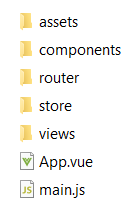
\includegraphics[height=5cm]{img/zdroj_kod_vue/src.png} }}
		\qquad
		\subfloat[\centering]{{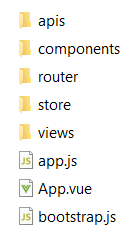
\includegraphics[height=5cm]{img/zdroj_kod_vue/js.png} }}
		\caption{Porovnání obsahu složek \textit{src} (a) a \textit{js} (b)}
		\label{fig:zdroj_kod_vue_rozdily}
	\end{figure}

	Každý soubor a složka ve zmíněném adresáři \textit{js} má určitý význam. Ty jsou představeny níže (soubor bootstrap.js byl již popsán výše). Další rozbor jednotlivých souborů ve zmíněných složkách je obsažen v dalších sekcích této práce.
	\begin{itemize}
		\item Složka \textit{apis} obsahuje prostředky pro komunikaci s API (tedy s backendem)
		\item Složka \textit{components} obsahuje všechny komponenty, které jsou využívány v celé aplikaci
		\item Složka \textit{router} obsahuje prostředky pro přesměrovávání a definování cest ve frontendové aplikaci
		\item Složka \textit{store} obsahuje nástroje pro držení dat ve webovém prohlížeči
		\item Složka \textit{views} obsahuje veškeré pohledy, na které se můžeme pomocí definované cesty dostat
		\item Soubor \textit{app.js} je kořenový soubor aplikace shromažďující všechny reference na ostatní soubory (zabaluje celou aplikaci)
		\item Soubor \textit{App.vue} je kořenová šablona, která přijímá pohledy na základě cesty, které poté vykresluje (tvoří aplikační kostru HTML)
	\end{itemize}

		\subsubsection{Souhrn využitých balíčků}\label{sec:fe_packages}
		Pro přehlednost je zde vytvořena kapitola shrnující vybrané externí balíčky, které byly do frontendové části přidány, a jejich základní účel a funkcionalita.
		
		\begin{itemize}
			\item Balíček \uv{@braid/vue-formulate} (dále jako VueFormulate) je použit pro veškeré formulářové prvky. Kromě zprostředkování hotových komponent pro jednotlivé elementy formuláře také nabízí např. validaci dat.
			\item Balíček \uv{vue-chartjs} (zastřešující populární balíček \uv{chart.js}) je použit pro grafické vyobrazení dat ve formě grafů.
			\item Balíček \uv{randomcolor} je použit pro generování náhodných barev (využito u grafů k dynamickému rozlišení dat)
			\item Balíček \uv{uuid} je použit pro generování unikátního identifikátoru (především funkce \textit{uuidv4}, např. u vytváření formuláře k označování vytvořených otázek)
			\item Balíček \uv{vue-js-modal} je použit k vytváření a správě modálních oken.
			\item Balíček \uv{vue-toasted} je použit pro zobrazování zpráv o průběhu různých činností (např. zobrazení chybových hlášek).
		\end{itemize}
	
		Dále frontend obsahuje reference na automaticky přidané balíčky, které nejsou předmětem této práce. Lze z nich ale vyjmout např. \uv{vuex} (správa držení dat v prohlížeči), \uv{vue-router} (správa cest mezi jednotlivými částmi aplikace - směrovač) či \uv{axios} (komunikace s API).
	
	\subsection{Komponenty}
	Komponenty jsou v podstatě \uv{díly k složení celé aplikace}. Díky nim nemusíme např. stránku pro vytvoření formuláře psát do jednoho nepřehledného a obrovského souboru, ale můžeme tento kód rozdělit. Výhodou také je, že když budeme tento komponentový styl zápisu kódu dodržovat, lze jeho části v jiných místech opětovně využít - předcházíme tím redundantnímu kódu, který zbytečně znepřehledňuje celý projekt. Všechny zmíněné komponenty jsou zapsány v souborech s koncovkou \textit{.vue} a disponují stejným jménem jako samotný soubor.
		
		\subsubsection{Základní komponenty} %Header, Loading, teor. App.vue
		Mezi základní komponenty jsou řazeny především ty, jejichž použití se opakuje v aplikaci nejčastěji - tedy \textit{Header} a \textit{Loading}. 
		
		Komponenta \textit{Header} slouží k vykreslení horního navigačního panelu s nabídkou dalších funkcionalit, který na základě přihlášení uživatele mění svůj obsah. Pokud není nikdo přihlášen, nabídka nabízí odkazy na přihlášení či registraci. Pokud se uživatel přihlásí, může se odsud dostat na stránku svého profilu, na vytvoření nového formuláře nebo se odhlásit ze svého účtu.
		
		Komponenta \textit{Loading} obsahuje jednoduchou animaci, která symbolizuje průběh načítání. Je využita v částech komponent a pohledů, kde je očekáván např. příjem nějakých dat z backendu, na který se musí čekat. Uživateli má vyobrazovat, že v aplikaci probíhá nějaká činnost.
		
		Dále zde lze zmínit i komponentu \textit{App} z kořenového adresáře frontendu, která již byla popsána v sekci \ref{sec:obecna_str_vuejs}. Lze dodat, že se v ní kromě předaných pohledů nachází i reference na komponentu \textit{Header} - ta musí být z podstaty věci vykreslena na všech cestách.
		
		\subsubsection{Komponenty elementů formuláře} %Elements, FormElement...*
		Tyto komponenty představují jednotlivé otázky a k ním příslušný vstup definovaný typem. Existují zde interaktivní komponenty elementů (použity např. ve vyobrazení formuláře k vyplnění) nebo komponenty statické (použity např. ve vyobrazení jednotlivých otázek při vytváření formuláře).
		
		Interaktivní komponenty elementů formuláře nalezneme v podsložce \textit{Elements} - zde se nachází tyto komponenty: \textit{BooleanInput}, \textit{DateInput}, \textit{NumberInput}, \textit{SelectInput} a \textit{TextInput} (vycházející z typů ze sekce \ref{sec:form_inputs_types}). Všechny tyto komponenty jsou si navzájem velmi podobné. Všechny využívají komponenty z balíčku \uv{VueFormulate}: \textit{FormulateInput} pro vykreslení samotné otázky a vytvoření vstupního pole podle datového typu pro odpověď (např. pro text je vygenerována oblast, do které lze vkládat textový řetězec) a \textit{FormulateErrors} pro výpis validační chyby (např. pokud má mít vkládaný text délku maximálně deset znaku a do oblasti vstupu je vložen text delší, tak se objeví chybové hlášení pod otázkou). V logické části jsou si taktéž všechny komponenty podobné - při jejich inicializaci se na základě přijmutích dat nastaví validační data a ID otázky, ke které samotná komponenta patří.
		
		Tyto interaktivní komponenty jsou poté zabaleny do dalších komponent. Komponenta \textit{FormElement} na základě příchozích dat (tj. typ otázky) vrací rodičovské komponentě \textit{FormElementsComponent} příslušný element formuláře rozebraný v předchozím odstavci. Zmíněná rodičovská komponenta poté figuruje především při vykreslování celého formuláře - má za úkol vykreslovat veškeré otázky formuláře s funkcí stránkování. Při inicializaci této komponenty se otázky nejprve rozdělí do příslušných polí, které představují stránky, na základě výskytu elementu nové stránky (tzn. pokud se při procházení všech elementů formuláře najde element nové stránky, tak je vytvořeno nové pole, do kterého se přesouvají další otázky). Po vzniku těchto polí představující stránky dojde k jejich vykreslení pomocí zmíněné komponenty \textit{FormElement}. Stránkování je zde zajištěno pomocí skrývání a odkrývání jednotlivých stránek pomocí CSS stylů ovládaných příslušnými tlačítky - takto to je řešeno kvůli udržení dat při přesunu na další stránku (nutné opatření kvůli zmíněnému balíčku k tvoření formulářových prvků).
		
		V rámci statických komponent zde existuje komponenta \textit{FormElementControl}. Ta slouží k vykreslování reprezentace otázek nebo elementu nové stránky v pohledech vytváření nebo úpravě formuláře. Jedná se o komponentu, která na základě předaného typu elementu (tj. otázka s příslušným typem nebo nová stránka) vrací příslušnou reprezentaci elementu (např. v případě textového vstupu vyobrazení textového pole, do kterého nelze vyplňovat, a samotné otázky). Při kliknutí na element otázky se objeví modální okno pro úpravu vybrané otázky - toto modální okno je popsáno dále v práci. U elementu nové stránky toto provést nelze, proto je zde připraven jen prokliknutelný text \uv{Remove}, který vysílá specifickou událost do rodičovské komponenty, která ho používá (slouží k odebrání elementu).
	
		\subsubsection{Modální okna} %Modals
		
		\subsubsection{Komponenty pro zobrazení výsledků} %ResultComponents
		
		\subsubsection{Komponenta karty formuláře} %FormCard
		
	
	\subsection{Komunikace s Laravel API}
	
	\subsection{Směrovač} %%Router
	
	\subsection{Držení dat v prohlížeči} %% Store
	
	\subsection{Pohledy}
		
		\subsubsection{Přihlašování a profil}
		
		\subsubsection{Domovská stránka}
		
		\subsubsection{Formulář}
		
		\subsubsection{Tvorba formuláře}
		
		\subsubsection{Úprava formuláře}
		
		\subsubsection{Souhrn informací o formuláři}
		
		\subsubsection{Výsledky formuláře}
		
		\subsubsection{Ostatní pohledy}
		%% not found, about
